The following plot compares all four implementations for various values of \texttt{x} and \texttt{m}. The number of clusters used for Snow and the number of threads used for OpenMP are both 8.\\

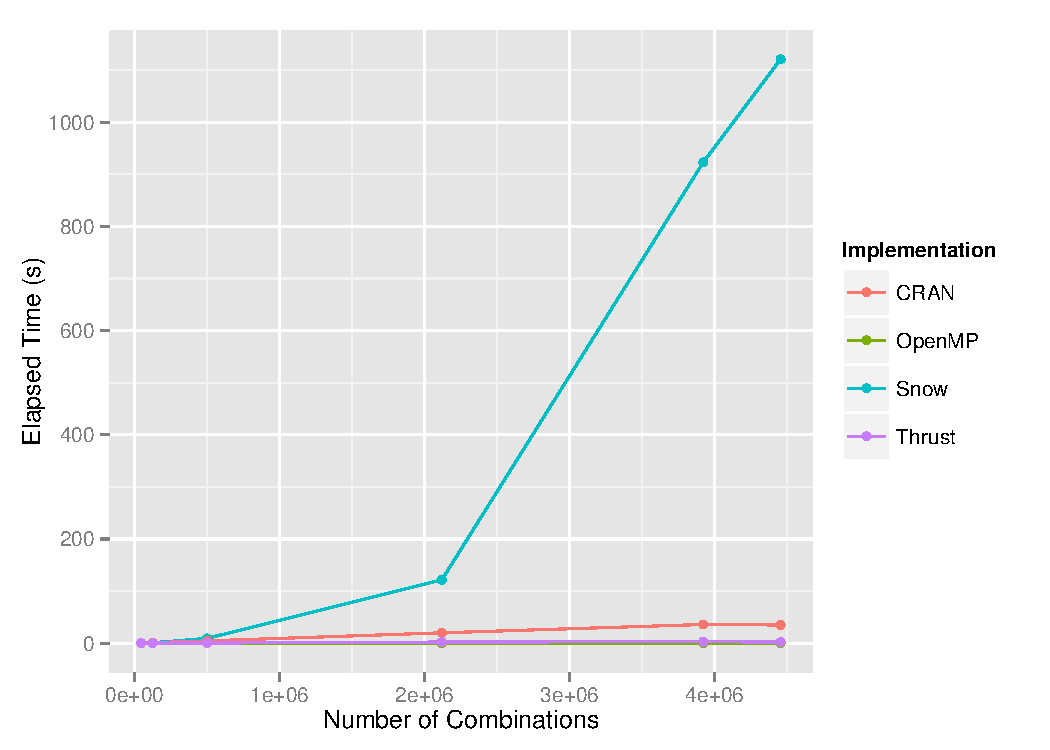
\includegraphics{all.pdf}\\
\null

Clearly, the Snow implementation is simply too slow. By excluding Snow, we can have a closer look on the speeds of the other three implementations:\\

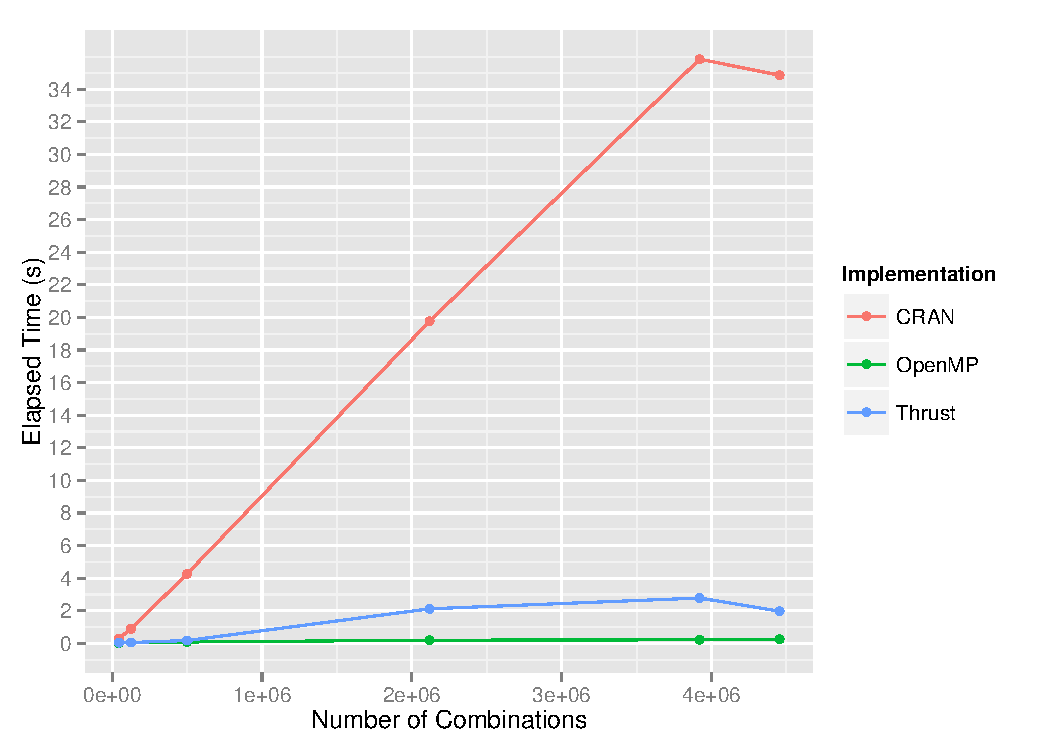
\includegraphics{withoutsnow.pdf}\\
\null

OpenMP and Thrust both massively improved the performance of \texttt{combn()} especially for large inputs. OpenMP was faster, and it also worked for even bigger inputs. We were able to get results for up to 75,287,520 combinations (\texttt{nCm(100, 5)}) in under 5 seconds. The differences in speeds between the OpenMP and Thrust implementations started to become quite significant at around 20,708,500 combinations (\texttt{nCm(500, 3)}). The Thrust program also started to have memory issues past this input size because of the limitations in the memory of the GPU. The speeds for OpenMP and Snow also didn't vary very significantly when using threads/nodes in the range of 6-10.\\
\null

